\chapter{Categories and Diagrams}

\todo{\chapabstract{}}

\paragraph{Prerequisites} Quantum Circuits $\cdot$

\section{Monoidal categories}
Monoidal categories provide an abstract structure for processes that are equipped with both sequential and parallel composition. One might be tempted to think of sequential composition as time-like and parallel composition as space-like, but this notion should be resisted as it can mislead in cases like, for example, quantum theory.  A process $f:A\to B$ is a \emph{morphism} from some input $A$ to output $B$. The $A$ and $B$ are called \emph{objects} and we sometimes say that $f$ is a morphism \emph{between} them. For morphisms $f:A\to B$ and $g:B\to C$, their \emph{composite} is a morphism $g\circ f:A\to C$. This data can be structured into a category, which then embodies the notion of sequential composition.\footnote{As a foundational comment, categories in the broadest mathematical literature do not in general require their objects and morphism to be sets. Categories where they do, as defined and used in this thesis, are \emph{small} categories. These details relate to the role categories can play in mathematical foundations \cite{mac1969one}.} We sometimes leave the objects of morphisms implicit when they can be inferred from context.

\begin{defn}
A \emph{category} \cat{C} is a set of objects $\objs{C}$ and a set of morphisms $\arrs{C}$ between them, such that for all $A,C,B,D\in \objs{C}$ and all $f:A\to B$, $g:B\to C$, $h:C\to D$ in $\arrs{C}$:
\begin{itemize}
\item for every pair of morphisms $f,g$, their composite $g\circ f$ is also in $\arrs{C}$;
\item composition is associative:
\begin{align}
h\circ(g\circ f) = (h\circ g)\circ f
\end{align}
\item for every object $A$ there is an $\idm{A}:A\to A$ in $\arrs{C}$ called the \emph{identity morphism} such that for all $f$:
\begin{align}
\idm{B}\circ f = f = f\circ\idm{A}.
\end{align}
\end{itemize}
\end{defn}

A category can thus be thought of as encoding processes where sequences can be associatively composed  and where we always have access to a ``do-nothing`` process, which is the identity morphism. Note that the objects of a category are somewhat superfluous, as they are in one-to-one correspondence with the identity morphisms. Due to this we refer interchangeable to an object and its identity morphism throughout. It is because categories are really focused on morphisms that we seem them as encoding a process theory.

Morphisms and their compositions can be represented in string diagrams:
\begin{equation}
\label{eq:composition}
f:A\to B := 
\begin{aligned}
\begin{tikzpicture}[xscale=\tikzxscale, yscale=\tikzyscale]

\node (1) at (0,2.5) {};
\node at (0.6,2.5) {$B$};
\node (2) [style=morphism] at (0,0) {$f$};
\node at (0.6,-2.5) {$A$};
\node (3) at (0,-2.5) {};

\draw [style = thick] (1.center) to (2.north);
\draw [style = thick] (2.south) to (3.center);

\end{tikzpicture}
\end{aligned}
\qquad
f \circ g := 
\begin{aligned}
\begin{tikzpicture}[xscale=\tikzxscale, yscale=\tikzyscale]

\node (0) at (0,2.5) {};
\node at (0.6,2.5) {$C$};
\node (1) [style=morphism] at (0,1.2) {$f$};
\node at (0.6,0) {$B$};
\node (2) [style=morphism] at (0,-1.2) {$g$};
\node at (0.6,-2.5) {$A$};
\node (3) at (0,-2.5) {};

\draw [style = thick] (0.center) to (1.north);
\draw [style = thick] (1.south) to (2.north);
\draw [style = thick] (2.south) to (3.center);

\end{tikzpicture}
\end{aligned}
\qquad
\idm{A} := 
\begin{aligned}
\begin{tikzpicture}[xscale=\tikzxscale, yscale=\tikzyscale]

\node (1) at (0,2.5) {};
\node at (0.6,2.5) {$B$};
\node at (0.6,-2.5) {$A$};
\node (3) at (0,-2.5) {};

\draw [style = thick] (1.center) to (3.center);

\end{tikzpicture}
\end{aligned}

\end{equation}
\noindent Here vertical connectivity, read from bottom to top, represents the flow of morphism composition.

\begin{defn}
A (strict)\footnote{Throughout this thesis we take monoidal categories to be strict, i.e. whose associators and unitors are identities.  In fact, every monoidal category is monoidally equivalent to a strict monoidal one \cite{joyal1993braided}.} \emph{monoidal category} is a category $\cat{C}$ equipped with a \emph{categorical tensor} $(-\otimes-):\cat{C}\times\cat{C}\to\cat{C}$ and a \emph{unit object} $I\in\objs{C}$ that obey:
\begin{equation}
(A\otimes B)\otimes C = A\otimes(B\otimes C),
\end{equation}
\begin{equation}
I\otimes A = A = A\otimes I.
\end{equation}
\end{defn}

Tensor composition is represented by horizontal adjoins and the identity object is the ``empty" diagram:
\begin{equation}
\label{eq:tensor}
f\otimes g := 
\begin{aligned}
\begin{tikzpicture}[xscale=\tikzxscale, yscale=\tikzyscale]

\node (1) at (0,2.5) {};
\node at (0.6,2.5) {$B$};
\node (2) [style=morphism] at (0,0) {$f$};
\node at (0.6,-2.5) {$A$};
\node (3) at (0,-2.5) {};

\draw [style = thick] (1.center) to (2.north);
\draw [style = thick] (2.south) to (3.center);

\node (12) at (2,2.5) {};
\node at (2.6,2.5) {$D$};
\node (22) [style=morphism] at (2,0) {$g$};
\node at (2.6,-2.5) {$C$};
\node (32) at (2,-2.5) {};

\draw [style = thick] (12.center) to (22.north);
\draw [style = thick] (22.south) to (32.center);


\end{tikzpicture}
\end{aligned}
=
\begin{aligned}
\begin{tikzpicture}[xscale=\tikzxscale, yscale=\tikzyscale]

\node (1) at (0,2.5) {};
\node at (0.6,2.5) {$B$};
\node (2) [style=morphism] at (0,1) {$f$};
\node at (0.6,-2.5) {$A$};
\node (3) at (0,-2.5) {};

\draw [style = thick] (1.center) to (2.north);
\draw [style = thick] (2.south) to (3.center);

\node (12) at (2,2.5) {};
\node at (2.6,2.5) {$D$};
\node (22) [style=morphism] at (2,-1) {$g$};
\node at (2.6,-2.5) {$C$};
\node (32) at (2,-2.5) {};

\draw [style = thick] (12.center) to (22.north);
\draw [style = thick] (22.south) to (32.center);


\end{tikzpicture}
\end{aligned}
\qquad \qquad \qquad
\idm{I} := 
\begin{aligned}
\begin{tikzpicture}[xscale=\tikzxscale, yscale=\tikzyscale]
\node at (1,0) {};
\node at (5,0) {};
\end{tikzpicture}
\end{aligned}

\end{equation}

\begin{defn}
\label{defn:state}
A \emph{state} of $A\in\objs{C}$ is a morphism $\ket{\psi}:I\to A$ drawn as
\begin{equation}
\label{eq:state}
\ket{\psi} :=  
\begin{aligned}
\begin{tikzpicture}[xscale=\tikzxscale, yscale=\tikzyscale]

\node (1) at (0,3) {};
\node at (0.6,3) {$A$};
\node (2) [style=state] at (0,1) {$\psi$};

\draw [style = thick] (1.center) to (2.center);

\end{tikzpicture}
\end{aligned}

\end{equation}
\end{defn}

\noindent The state morphism can be thought of as a preparation process to create that state.

\section{Symmetric monoidal categories}

\begin{defn}
A monoidal category is \emph{symmetric} (an SMC) when it has a isomorphism
$\sigma_{A,B}:A\otimes B\to B\otimes A$ that satisfies the following graphical equations:
\begin{equation}
\label{eq:symmetry}
\sigma_{A,B} := 
\begin{aligned}
\begin{tikzpicture}[xscale=1.2*\tikzxscale, yscale=\tikzyscale]

\node (0) at (-1, 1) {};
\node (1) at (1, 1) {};
\node (2) at (1, -1) {};
\node (3) at (-1, -1) {};
\node (4) at (0, -0) {};

\draw [bend left, looseness=1.00] (3.center) to (4.center);
\draw [bend right, looseness=1.00] (4.center) to (1.center);
\draw [bend left, looseness=1.00] (4.center) to (0.center);
\draw [bend left, looseness=1.00] (4.center) to (2.center);

\end{tikzpicture}
\end{aligned}
\qquad \qquad
\begin{aligned}
\begin{tikzpicture}[xscale=1.2*\tikzxscale, yscale=\tikzyscale]

\node (0) at (-1, 1) {};
\node (1) at (1, 1) {};
\node (2) at (1, -1) {};
\node (3) at (-1, -1) {};
\node (4) at (0, 0) {};
\node (02) at (-1, 3) {};
\node (12) at (1, 3) {};
\node (22) at (1, 1) {};
\node (32) at (-1, 1) {};
\node (42) at (0, 2) {};

\draw [bend left, looseness=1.00] (3.center) to (4.center);
\draw [bend right, looseness=1.00] (4.center) to (1.center);
\draw [bend left, looseness=1.00] (4.center) to (0.center);
\draw [bend left, looseness=1.00] (4.center) to (2.center);

\draw [bend left, looseness=1.00] (32.center) to (42.center);
\draw [bend right, looseness=1.00] (42.center) to (12.center);
\draw [bend left, looseness=1.00] (42.center) to (02.center);
\draw [bend left, looseness=1.00] (42.center) to (22.center);

\end{tikzpicture}
\end{aligned}
=
\begin{aligned}
\begin{tikzpicture}[xscale=1.2*\tikzxscale, yscale=\tikzyscale]

\node (0) at (0,-1) {};
\node (1) at (0,3) {};
\node (2) at (1,-1) {};
\node (3) at (1,3) {};

\draw (0.center) to (1.center);
\draw (2.center) to (3.center);

\end{tikzpicture}
\end{aligned}

\end{equation}
\begin{equation}
\label{eq:symmetry2}
\sigma_{A,B} := 
\begin{aligned}
\begin{tikzpicture}[xscale=1.2*\tikzxscale, yscale=\tikzyscale]

\node (0) at (-1, 1) {};
\node (1) at (1, 1) {};
\node (2) at (1, -1) {};
\node (3) at (-1, -1) {};
\node (4) at (0, -0) {};

\draw [bend left, looseness=1.00] (3.center) to (4.center);
\draw [bend right, looseness=1.00] (4.center) to (1.center);
\draw [bend left, looseness=1.00] (4.center) to (0.center);
\draw [bend left, looseness=1.00] (4.center) to (2.center);

\end{tikzpicture}
\end{aligned}
\qquad \qquad
\begin{aligned}
\begin{tikzpicture}[xscale=1.2*\tikzxscale, yscale=\tikzyscale]

\node (0) at (-1, 1) {};
\node (1) at (1, 1) {};
\node (2) at (1, -1) {};
\node (3) at (-1, -1) {};
\node (4) at (0, 0) {};
\node (02) at (-1, 3) {};
\node (12) at (1, 3) {};
\node (22) at (1, 1) {};
\node (32) at (-1, 1) {};
\node (42) at (0, 2) {};

\draw [bend left, looseness=1.00] (3.center) to (4.center);
\draw [bend right, looseness=1.00] (4.center) to (1.center);
\draw [bend left, looseness=1.00] (4.center) to (0.center);
\draw [bend left, looseness=1.00] (4.center) to (2.center);

\draw [bend left, looseness=1.00] (32.center) to (42.center);
\draw [bend right, looseness=1.00] (42.center) to (12.center);
\draw [bend left, looseness=1.00] (42.center) to (02.center);
\draw [bend left, looseness=1.00] (42.center) to (22.center);

\end{tikzpicture}
\end{aligned}
=
\begin{aligned}
\begin{tikzpicture}[xscale=1.2*\tikzxscale, yscale=\tikzyscale]

\node (0) at (0,-1) {};
\node (1) at (0,3) {};
\node (2) at (1,-1) {};
\node (3) at (1,3) {};

\draw (0.center) to (1.center);
\draw (2.center) to (3.center);

\end{tikzpicture}
\end{aligned}

\end{equation}
\begin{equation}
\label{eq:symmetry3}
\begin{aligned}
\begin{tikzpicture}[xscale={\tikzxscale}, yscale={\tikzyscale}]
                \node [style=morphism] (0) at (-1, -0) {$f$};
                \node [style=morphism] (1) at (1, -0) {$g$};
                \node (2) at (1, -1) {};
                \node (3) at (-1, -1) {};
                \node (4) at (0, 1.2) {};
                \node (5) at (-1, 2) {};
                \node (6) at (1, 2) {};

                \draw [bend right, looseness=1.00] (5.center) to (4.center);
                \draw [bend left, looseness=1.00] (4.center) to (1.north);
                \draw [bend left, looseness=1.00] (6.center) to (4.center);
                \draw [bend right, looseness=1.00] (4.center) to (0.north);
                \draw (0.south) to (3.center);
                \draw (2.center) to (1.south);
\end{tikzpicture}
\end{aligned}
\;=\;
\begin{aligned}
\begin{tikzpicture}[xscale={\tikzxscale}, yscale={\tikzyscale}]
                \node [style=morphism] (0) at (-1, 1) {$g$};
                \node [style=morphism] (1) at (1, 1) {$f$};
                \node (2) at (1, 2) {};
                \node (3) at (-1, 2) {};
                \node (4) at (0, -0.2) {};
                \node (5) at (-1, -1) {};
                \node (6) at (1, -1) {};

                \draw [bend left, looseness=1.00] (5.center) to (4.center);
                \draw [bend right, looseness=1.00] (4.center) to (1.south);
                \draw [bend right, looseness=1.00] (6.center) to (4.center);
                \draw [bend left, looseness=1.00] (4.center) to (0.south);
                \draw (0.north) to (3.center);
                \draw (2.center) to (1.north);
\end{tikzpicture}
\end{aligned}

\end{equation}
\end{defn}
\noindent where Equation \ref{eq:symmetry3} is the naturality of $\sigma$.

\begin{examples}
The following are some examples of SMC's:
\begin{itemize}
\item \cat{FHilb}, the category where objects are finite dimensional Hilbert spaces; morphisms are linear maps; the categorical tensor is the tensor product; the identity object $I=\mathbb{C}$.
\end{itemize}
\end{examples}

\begin{theorem}{\cite[Thm 2.3]{joyal1991geometry}}
A well-formed equation between morphisms in a symmetric monoidal category follows from the axioms if and only if it holds in the graphical language up to isomorphism of diagrams.
\end{theorem}

\subsection{Symmetric monoidal categories \&\ quantum circuits}
This thesis applies the graphical calculi for SMC's to the study of protocols and algorithms for and inspired by quantum theory. For this, it can be useful to think of the SMC graphical calculus as mathematical scaffolding that underlies quantum circuit diagrams. See Figure \ref{fig:QCDSMC} for an example. Note that state preparation is included as a part of the categorical diagram while it is extra labeling in the quantum circuit. In $\cat{FHilb}$ we have $I=\mathbb{C}$, and so the states, by Definition \ref{defn:state}, of some Hilbert space $\Hsp$ are exactly maps $\ket{\psi}:\mathbb{C}\to\Hsp$. These are recognized as the usual quantum state vectors $\ket{\psi}\in\Hsp$. This allows states to be manipulated graphically as well, to advantages discussed later. In uncovering SMC scaffolding of quantum circuits, we are able to improve it, introducing techniques to reason graphically about more advanced structures and that better capture the salient features of these processes. We cover these new features in Chapter \ref{chap:cqm}.

\begin{figure}[t]
\label{fig:QCDSMC}
\begin{equation*}
\begin{aligned}
\Qcircuit @C=1em @R=.7em {
&& {/} \qw & \multigate{1}{U} & \qw & \multigate{2}{f} & \qw \\
$\ket{1}$ && \qw & \ghost{U}& \qw & \ghost{f} & \qw \\
$\ket{0}$ && \gate{H} & \qw & \qw & \ghost{f} & \qw 
}
\end{aligned}
\qquad\qquad\qquad
\begin{aligned}
\begin{tikzpicture}[xscale=1, yscale=0.8]
        \node (0) at (-1, -2) {};
        \node [style=state] (1) at (1, -2) {$0$};
        \node [style=state] (2) at (0, -2) {$1$};
        \node [style=morphism] (3) at (1, -1) {$H$};
        \node [style=morphism, xscale=3] (4) at (-0.5, -0) {};
        \node [style=morphism, xscale=5] (5) at (0, 1.25) {};
        \node (7) at (0, -0.2) {};
        \node (8) at (-1, -0.2) {};
        \node (9) at (-1, 0.25) {};
        \node (10) at (0, 0.25) {};
        \node (11) at (1, 0.25) {};
        \node (12) at (1, 1.1) {};
        \node (13) at (0, 1.1) {};
        \node (14) at (-1, 1.1) {};
        \node (15) at (-1, 1.4) {};
        \node (16) at (0, 1.4) {};
        \node (17) at (1, 1.4) {};
        \node (18) at (0, 2) {};
        \node (19) at (1, 2) {};
        \node (20) at (-1, 2) {};
        \node (21) at (-1, -2.5) {$\Hsp_N$};
        \node (23) at (-1, 2.5) {$\Hsp_2$};
        \node (24) at (0, 2.5) {$\Hsp_2$};
        \node (25) at (1, 2.5) {$\Hsp_2$};
        \node (26) at (0, 1.24) {$f$};
        \node (27) at (-0.5, -0.05) {$U$};

        \draw (0.center) to (8.south);
        \draw (7.south) to (2);
        \draw (1) to (3.south);
        \draw (3.north) to (11.center);
        \draw (11.center) to (12.south);
        \draw (19.center) to (17.north);
        \draw (16.north) to (18.center);
        \draw (20.center) to (15.north);
        \draw (14.south) to (9.center);
        \draw (13.south) to (10.center);
\end{tikzpicture}
\end{aligned}
\end{equation}


\caption[Comparison of quantum circuits and symmetric monoidal diagrams]{On the left we have a quantum circuit (read left to right) and its corresponding categorical diagram in \cat{FHilb} on the right (read bottom to top). In both depictions, the boxes are linear maps and the wires are Hilbert spaces. In quantum circuits these are implicitly qubits, with a slash used to denote products of qubits. In the categorical diagram we explicitly write spaces.}
\end{figure}

\subsection{Other Categorical Definitions}

We make use of several other standard categorical concepts, whose definitions are reproduced here.

\begin{defn}
Given a category $\cat{C}$ and $A,B\in\objs{C}$, the \emph{homset} Hom$(A,B)$ is the set of arrows in the category $f:A\to B$.
\end{defn}

We can think of Hom$(A,B)$ as all the processes that input system $A$ and output $B$. Sometimes, to specify the category, we write $\cat{C}(A,B)$ for the homset Hom$(A,B)$ in $\cat{C}$.

As we often consider the relationship between categories, we introduce the notion of a structure preserving map between categories that is called a functor.

\begin{defn}
Given two categories \cat{C} and \cat{D} a \emph{functor} $F:\cat{C}\to\cat{D}$ consists of
\begin{enumerate}
\item A mapping on objects $F:\objs{C}\to\objs{D}::A\mapsto F(A)$
\item A mapping on arrows $F:\cat{C}(A,B)\to\cat{D}(F(A),F(B))::f\mapsto F(f)$ that preserves composition and identities, i.e. 
\begin{enumerate}
\item For $f:A\to B$ and $g:B\to C$ then $F(g\circ f) = F(g)\circ F(f)$
\item $F(1_A)=1_{F(A)}$
\end{enumerate}
\end{enumerate}
\end{defn}

\section{Further Reading}
Monoidal and symmetric monoidal categories were introduced as ``categories with multiplication" by MacLane in \cite{maclane1963natural} and later formalized as string diagrams by \cite{joyal1991geometry}. There are other examples, besides quantum information, where diagrammatic concepts in computer science and physics have been formalized using them.  In general, this approach is most useful when there are processes have both a natural diagrammatic (\emph{geometric}) presentation, but that also have an \emph{algebraic} interpretation.

In physics, Penrose's tensor notation \cite{penrose1971applications} is, in modern language, precisely the diagrammatic representation of the symmetric monoidal category $\cat{FVect}$ of finite dimensional vector spaces and linear maps. Feynman diagrams are representations of morphisms in the symmetric monoidal category of positive energy representations of the Poincar\'{e} group \cite{baez2009prehistory}. The symmetric (and braided) monoidal category framework is an important foundation for $n$-dimensional topological quantum field theories (symmetric monoidal functors $T:\cat{nCob}\to \cat{FVect}$) \cite{atiyah1988topological}. In fact, two-dimensional TQFT's are equivalent to commutative Frobenius algebras, which we introduce later in \todo{DEFINITION cFAlg} \cite{abrams1996two,kock2004frobenius}. This perspective also plays an important role in the study of generalized knot invariants \cite{reshetikhin1990ribbon} and quantum groups \cite{baez2009prehistory}. 

We also find example in computer science and control theory. Petri nets (Figure~\ref{petri}) have been connected to linear logic through their connection with monoidal categories \cite{abramsky2008petri,marti1989petri,sassone1998axiomatization}.
\begin{figure}[t]
\label{fig:petri}
\begin{align*}
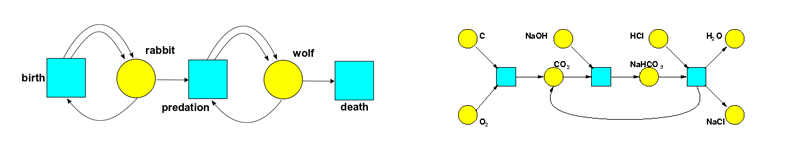
\includegraphics[width=\textwidth]{images/petri.png}
\end{align*}
\caption{Two examples of Petri nets.  On the left is a Petri net for a predator prey system and on the right is one for a chemical reaction. Figure reproduced with permission from \cite{petriBlog}.}
\end{figure}
Each Petri net, by closure under sequential and parallel composition makes a suitable kind of symmetric monoidal category \cite{marti1989petri,meseguer1990petri}. Categories in Control. Reversible flow circuits.  Electrical
circuits. Cannabalize Kissinger/Vladimir's introductions.

Note that monoidal categories are themselves coherent for planar isotopy \cite{joyal1991geometry}. Indeed the coherence of many of these graphical languages can be regarded are geometric isotopies in higher dimensions, e.g. coherence for SMC's is up to a 4-dimensional isotopy \cite{selinger2011survey}. This establishes a hierarchy of diagrams that ...

A general reference for the connections between computation, topology, and physics that emerge from symmetric monoidal categories is \cite{baez2011physics}.

